\begin{pa} \label{PA:5.2}
Consider the function $A$ defined by the rule
$$A(x) = \int_1^x f(t) \, dt,$$
where $f(t) = 4-2t$.
%\begin{figure}[h]
%\begin{center}
%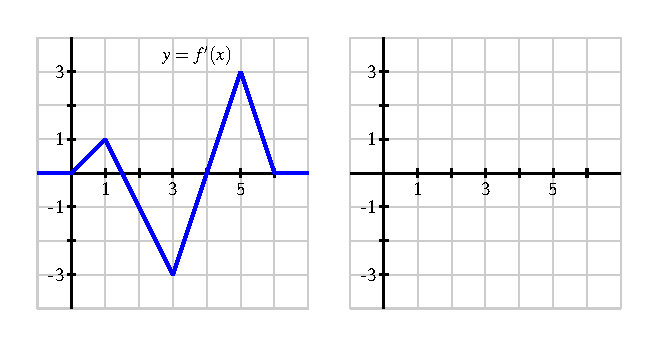
\includegraphics{figures/5_1_PA1.eps}
%\caption{At left, the graph of $y = f'(x)$; at right, axes for plotting $y = f(x)$.} \label{F:5.1.PA1}
%\end{center}
%\end{figure}
\ba
	\item Compute $A(1)$ and $A(2)$ exactly.
	\item Use the First Fundamental Theorem of Calculus to find an equivalent formula for $A(x)$ that does not involve integrals.  That is, use the first FTC to evaluate $\int_1^x (4-2t) \, dt$.
	\item Observe that $f$ is a linear function; what kind of function is $A$?
	\item Using the formula you found in (b) that does not involve integrals, compute $A'(x)$.
	\item While we have defined $f$ by the rule $f(t) = 4-2t$, it is equivalent to say that $f$ is given by the rule $f(x) = 4 - 2x$.  What do you observe about the relationship between $A$ and $f$?
\ea
\end{pa} 
\afterpa